\chapter{JDart et exécution concolique}
  \paragraph{}
    L'idée générale est de rendre la tâche de tester des Applets Java Card moins penible et plus effective que possible.
    Pour celà nous optons pour l'utilisation de l'execution concolique comme une technique d'analyse ce qui permet de rendre 
    le system à tester moins obscure et plus predictible surtout quand on est face à des systemes complexes
    et qui nécessitent des méthodes plus avancées qu'un simple teste unitaire.
  \paragraph{}
    \textbf{JDart \footnote{JDart : https://github.com/psycopaths/jdart}} est un outil qui permet d'utiliser l'execution concolique comme une technique de teste pour les applications Java.
    \newline
    Il se présente sous forme d'une extension de \gls{JPF} un outil créé par le NASA afin de tester ses applications y compris les programmes executés sur ses robots astromobiles.
  \section{Exploration des chemins et l'execution concolique}
    \subsection{Java Path Finder: Exploration des chemins}
      \nocite{JPF}
      \paragraph{}
	\gls{JPF} est un outil de verification des modéles d'état pour le bytecode Java,
	donc \gls{JPF} est en fait une \gls{VM} qui execute le programme donné en entrée autant de fois que nécessaire
	afin d'explorer chaque chemin qu'il contient.
	Tout au long de ce processus, \gls{JPF} collecte les anomalies rencontrés tel que l'interblocage des threads et les exceptions non traités,
	puis il génére un rapport contenant les traces qui ménent à ces anomalies.
	
	\begin{figure}[H]
	  \centering
	    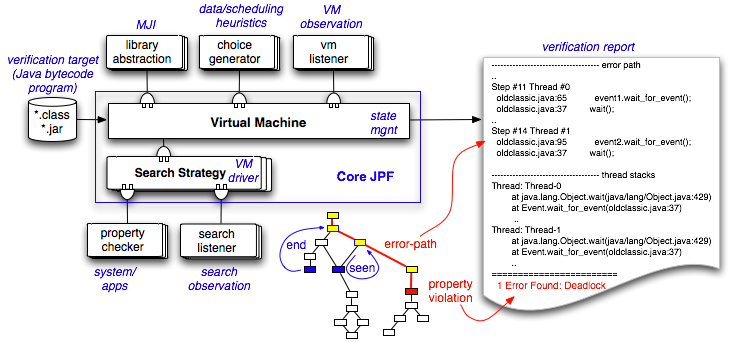
\includegraphics[scale=0.5]{images/jpf-model.png}
	  \caption{modéle d'opération de \gls{JPF}}
	\end{figure}
      \paragraph{}
	\gls{JPF} ne se limite pas à simplement detecter les erreurs d'un programme, en effet il effectue la vérification des modéles,
	C'est un outil qui permet de simuler le non-determinisme. Certain aspect ne peuvent pas être controller par de simples testes
	et exigent l'assistance d'une \gls{VM}.
	Cependant, en essayant d'explorer et executer tous les chemins au sein d'un programme, le nombre d'execution nécessaire peut
	croître d'une maniére exponentielle (On parle du problème d'explosion d'état). Pour resoudre ce problème, \gls{JPF} réalise une
	correspondance d'état, c'est un mecanisme qui permet de comparer l'état actuel en un n\oe{}ud à des états déjà connus, dans le cas où l'état
	a été verifié \gls{JPF} est capable d'éffectuer un retour arrière à la position précedente la plus proche où un chemin inexploré existe et 
	restaure l'état du programme à tester à cette position.
	
      \begin{figure}[H]
	\centering
	  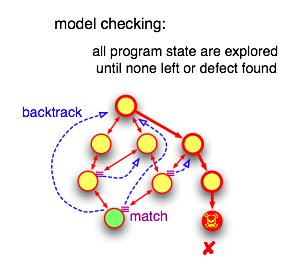
\includegraphics[scale=0.5]{images/jpf-model-checking.png}
	\caption{Vérification du modéles}
      \end{figure}
      
      \paragraph{}
	La vérification des modéles (\textit{Model Checking}) ne dépend pas sur des conjectures. En théorie si une anomalie est présente dans le programme à tester
	alors la vérification des modéles la trouvera, puisque c'est une méthode qui explore d'une maniére exhausive tous les comportements possible du systeme,
	d'où vient l'éfficacité du \textit{Model Checking}.
    \subsection{JDart: Exécution concolique}
	
    
      
  \section{La VM JAVA, La VM du JPF et la VM JavaCard}
  \section{Tester des applets JavaCard}
  \paragraph{}
    Java Path Finder connu comme le couteau Suisse de la verification Java,
    est en effet un des outis de teste les plus evolués pour les applications Java,
    grâce à son extensibilité et à son abilité de supporter et interger de nouvelle extensions.
    Cependant, la majorité des extensions ne sont pas destinés à être executer sur des systemes JavaCard.